\documentclass[11pt,a4paper]{article}
\usepackage{amsmath, amsthm, mathtools, fontenc, graphicx}
\usepackage{subcaption}
\usepackage{etex,datetime,setspace,latexsym,amssymb,amsmath,amsthm}
\usepackage{fancybox,dialogue,float,wrapfig,enumerate,microtype}
\usepackage{verbatim,xcolor,multicol,titlesec,tabularx,mdframed}
\usepackage{ circuitikz }


\usepackage[utf8]{inputenc}
\usepackage[pdftex]{hyperref}
\usepackage[margin=2cm,bottom=3cm,footskip=15mm]{geometry}
\parindent0cm
\parskip0.5em

\usepackage{tikz}
\usetikzlibrary{arrows,trees,positioning,shapes,patterns}
\usetikzlibrary{intersections,calc,fpu,decorations.pathreplacing}

\usepackage[T1]{fontenc} % better fonts

% Haskell code listings in our own style
\usepackage{listings,color}
\definecolor{lightgrey}{gray}{0.35}
\definecolor{darkgrey}{gray}{0.20}
\definecolor{lightestyellow}{rgb}{1,1,0.92}
\definecolor{dkgreen}{rgb}{0,.2,0}
\definecolor{dkblue}{rgb}{0,0,.2}
\definecolor{dkyellow}{cmyk}{0,0,.7,.5}
\definecolor{lightgrey}{gray}{0.4}
\definecolor{gray}{gray}{0.50}
\lstset{
  language        = Haskell,
  basicstyle      = \scriptsize\ttfamily,
  keywordstyle    = \color{dkblue},     stringstyle     = \color{red},
  identifierstyle = \color{dkgreen},    commentstyle    = \color{gray},
  showspaces      = false,              showstringspaces= false,
  rulecolor       = \color{gray},       showtabs        = false,
  tabsize         = 8,                  breaklines      = true,
  xleftmargin     = 8pt,                xrightmargin    = 8pt,
  frame           = single,             stepnumber      = 1,
  aboveskip       = 2pt plus 1pt,
  belowskip       = 8pt plus 3pt
}
\lstnewenvironment{code}[0]{}{}

% only shown, not compiled:
\lstnewenvironment{showCode}[0]{\lstset{numbers=none}}{}

% only compiled, not shown:
\newcommand{\hide}[1]{}

% will the real phi please stand up
\renewcommand{\phi}{\varphi}

\newcommand{\gor}{\mathbin{\rotatebox[origin=c]{-90}{$ \geqslant $}}}


% load hyperref as late as possible for compatibility
\usepackage[pdftex]{hyperref}
\hypersetup{
  colorlinks = true,
  pdfborder = {0 0 0},
  breaklinks = true,
  linktoc = all,
  linkcolor = blue,
  urlcolor = magenta
}
\pdfinfoomitdate=1
\pdftrailerid{}
\pdfsuppressptexinfo15

\newcommand{\mycomment}[1]{}

\title{Model Checking BSML}
\author{N. Cohen, T. Coroneo, V. Iyer, G. Kaminer, and L. Madison}
\date{\today}
\hypersetup{pdfauthor={FP 2025, Group 3}, pdftitle={Model Checking BSML}}

\setlength{\parskip}{10pt plus 1pt minus 1pt}

\DeclareMathOperator{\botbot}{\rotatebox{90}{$\models$}}
\DeclareMathOperator{\toptop}{\raisebox{0pt}[0pt][0pt]{\rotatebox[origin=c]{270}{$\models$}}}

\begin{document}

\maketitle

\begin{abstract}
Bilateral State-based Modal Logic (BSML) was introduced in \cite{Aloni2022} to model Free-Choice (\textit{FC}) and related inferences which arise from speakers' distaste for
interpretations that verify a sentence by empty configuration (\textit{neglect-zero tendency}). To preclude such empty configurations, BSML uses state-based semantics (propositions evaluated at sets of worlds rather than individual worlds) and extends basic modal logic with a pragmatic enrichment function $[]^+$ which requires supporting states to be nonempty.
We implement an explicit model checker for BSML and use this to verify some properties, like Free-Choice inference, as described in \cite{Aloni2024}.
\end{abstract}

\tableofcontents

\clearpage

\section{Introduction}
This section outlines the motivation for BSML by walking through a simple example from \cite{Aloni2022}. Readers interested only in the implementation can safely skip this section.

\subsection{Motivating example}
Free-Choice (\textit{FC}) inferences are instances of a disjunctive sentence (``or'') unexpectedly yielding a conjunctive reading (``and''). In the following example, a modalized disjunction (1) yields a conjunction of modals (2).

\begin{enumerate}
\item $\lozenge(b\vee c)$ You may go to the beach \textbf{or} to the cinema
\item $\lozenge b \wedge \lozenge c$ You may go to the beach \textbf{and} you may go to the cinema
\end{enumerate}

Aloni \cite{Aloni2022} posits that speakers interpret a sentence by identifying structures of reality that reflect it. Such a structure, or ``information state'', is a set of possible worlds.

In our disjunction, there are four associated worlds:

\begin{enumerate}
\item $W_{bc}$ in which both $b$ and $c$ are true (you go to both the beach and the cinema)
\item $W_b$ in which $b$ is true (you go to the beach)
\item $W_c$ in which $c$ is true (you go to the cinema)
\item $W_z$ in which neither $b$ nor $c$ is true (you don't go anywhere)
\end{enumerate}

 We can use BSML to model the information states (i.e. sets of worlds) in which the disjunction $b\vee c$ is assertable (or rejectable). A disjunction $\varphi\vee\psi$ is assertable in a state $s$ if $s$ is the union of two substates $t$ and $u$, where $\varphi$ is assertable in $t$ and $\psi$ is assertable in $u$.

\begin{enumerate}
\item Where state $s_1$ is the union of $W_b$ and $W_c$, $b\vee c$ is assertable since $b$ is assertable in $W_b$ and $c$ is assertable in $W_c$
\item Where state $s_2$ is the union of $W_{bc}$ and $W_b$ (or $W_{bc}$ and $W_c$), $b\vee c$ is assertable since $b$ is assertable in $W_b$ and $c$ is assertable in $W_{bc}$
\item Where state $s_3$ is the union of $W_b$ and the empty set (or $W_c$ and the empty set), $b\vee c$ is assertable since


since each of the
disjuncts is assertable in a substate. $b$ is assertable in $W_b$, and $c$ is supportable in the empty state.
\item In a state consisting of $W_z$ and $W_b$ (and any other state which includes $W_z$), $b\vee c$ is
\textit{not} assertable because in $W_z$ both $b$ and $c$ are false, so no substate containing $W_z$ would allow assertion of $b$ or $c$.
\end{enumerate}

So, among the four types of states, $b\vee c$ is assertable in all but the last. This is a problem, because if
$b\vee c$ is assertable in a state consisting only of $W_b$ (or a state consisting of only $W_c$) then we have
that $\Diamond(b\vee c)$ is true while $\Diamond b \wedge \Diamond c$ is false, so the FC inference fails. The
problematic state, then, is the zero-model: one of the states which it uses to satisfy the disjunction is the
empty state.

How do we account for FC inferences then? Aloni argues pragmatically that a speaker would not consider the
zero-model as one of the candidate states. Neglecting the zero model then, the FC inference would hold
because the only states that would support $b\vee c$ would be (1) or (2). To model neglect-zero (to make
sure that $b\vee c$ is not assertable in the zero-model), we require that to satisfy a disjunction, the state
must be the union of two non-empty substates rather than just the union of two substates.
This is modelled by enriching formulas using a \emph{pragmatic enrichment function} which conjuncts to each subformula a non-emptiness atom (\verb|NE|), which requires supporting states to be inhabited.

The enrichment of $b \vee c$ (denoted $[b\vee c]^+$) is no longer assertable in a state consisting of only $W_b$
(or a state consisting of only $W_c$) since \verb|NE| would not be assertable in any substates that could (vacuously) support $c$.
Finally then, since the only states in which the enriched disjunction holds are (1) and (2), the FC inference holds.

\subsection{Our contribution}

This report details our implementation of an explicit model checker for BSML.
In the last section, we create a framework for writing Natural Deduction style
proofs for BSML in Haskell.

Developing model-checkers is useful for any logic - it helps us understand quickly whether a formula is true on a particular model (while removing any human
error involved in this process), and also makes it easy for the user to check the validity of a class of formulas on a class of models quickly.
The goal is to ensure model-checkers are accurate and efficient: while in BSML the latter criterion is hard to achieve on account of the unique
semantics of the logic, we have tried to ensure that the model-checker is as efficient as possible while remaining sound.

Our implementation for Natural Deduction can be used as a (quite primitive for now) interactive theorem prover for BSML.
Representing these proofs is also the first step to potentially building a functional automated theorem prover for the language. As with model-checkers, this makes the
job of anyone working in the field easier as they may now systematically verify the correctness of their proofs. Our representation of Natural Deduction is built by creating a new \verb|Proof| type, and ensuring that the only
way one can get from one proof to another is by following the axiomatization of BSML outlined in \cite{Aloni2024}.
​

\section{Model checking BSML}\label{sec:BSML}

This section describes the implementation of the explicit model checker for BSML. 
More precisely, we will focus on $\mathrm{BSML}^{\gor}$, an extension of BSML with so-called \emph{global disjunction}. 
This extension was not chosen for conceptual reasons, but merely to make the implementation of Natural Deduction more palatable, as we will see later. 
Throughout this report, we will not need to differentiate between BSML and $\mathrm{BSML}^{\gor}$, so we will be somewhat sloppy and simply write BSML for our language. 


\input{lib/Syntax.lhs}

\input{lib/Semantics.lhs}


\subsection{Verifying basic properties}

\begin{figure}[!h]
    \centering
    \begin{subfigure}[b]{0.32\textwidth}
        \centering
        \resizebox{\linewidth}{!}{%
            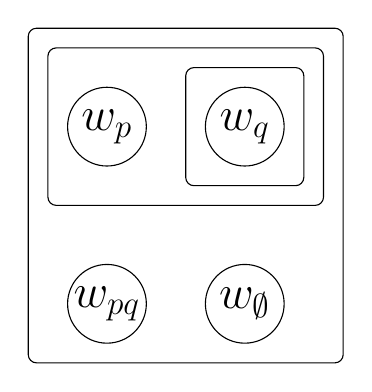
\begin{tikzpicture}[every node/.style={font=\LARGE}]
                \draw (2.5,13.75) circle (0.5cm) node {$w_p$};
                \draw (4.25,13.75) circle (0.5cm) node {$w_q$};
                \draw (2.5,11.5) circle (0.5cm) node {$w_{pq}$};
                \draw (4.25,11.5) circle (0.5cm) node {$w_{\emptyset}$};
                \draw [rounded corners=3.0] (1.75,14.75) rectangle (5.25,12.75);
                \draw [rounded corners=3.0] (3.5,14.5) rectangle (5,13);
                \draw [rounded corners=3.0] (1.5,15) rectangle (5.5,10.75);
            \end{tikzpicture}%
        }
        \caption{Example 3a}
        \label{fig:3a}
    \end{subfigure}
    \hfill
    \begin{subfigure}[b]{0.32\textwidth}
        \centering
        \resizebox{\linewidth}{!}{%
            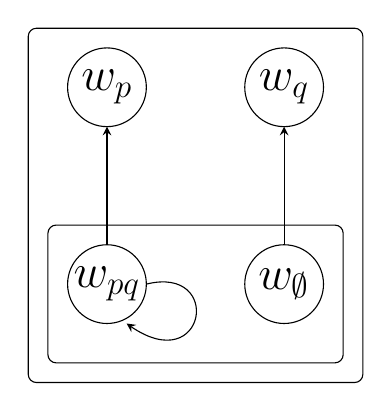
\begin{tikzpicture}[every node/.style={font=\LARGE}]
                \draw (0.75,14.25) circle (0.5cm) node {$w_p$};
                \draw (3,14.25) circle (0.5cm) node {$w_q$};
                \draw (0.75,11.75) circle (0.5cm) node {$w_{pq}$};
                \draw (3,11.75) circle (0.5cm) node {$w_{\emptyset}$};
                \draw [rounded corners=3.0] (0,10.75) rectangle (3.75,12.5);
                \draw [rounded corners=3.0] (-0.25,15) rectangle (4,10.5);
                \draw [->, >=stealth] (1.25,11.75) .. controls (2.25,12) and (2,10.5) .. (1,11.25);
                \draw [->, >=stealth] (0.75,12.25) -- (0.75,13.75);
                \draw [->, >=stealth] (3,12.25) -- (3,13.75);
            \end{tikzpicture}%
        }
        \caption{Example 3b}
        \label{fig:3b}
    \end{subfigure}
    \hfill
    \begin{subfigure}[b]{0.32\textwidth}
        \centering
        \resizebox{\linewidth}{!}{%
            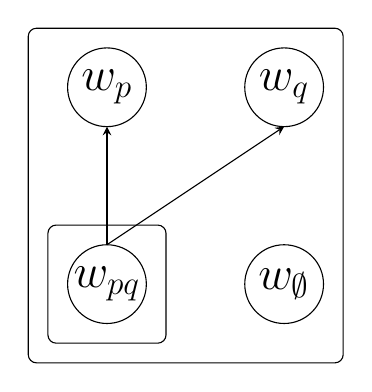
\begin{tikzpicture}[every node/.style={font=\LARGE}]
                \draw (0.75,14.25) circle (0.5cm) node {$w_p$};
                \draw (3,14.25) circle (0.5cm) node {$w_q$};
                \draw (0.75,11.75) circle (0.5cm) node {$w_{pq}$};
                \draw (3,11.75) circle (0.5cm) node {$w_{\emptyset}$};
                \draw [rounded corners=3.0] (0,11) rectangle (1.5,12.5);
                \draw [rounded corners=3.0] (-0.25,15) rectangle (3.75,10.75);
                \draw [->, >=stealth] (0.75,12.25) -- (0.75,13.75);
                \draw [->, >=stealth] (0.75,12.25) -- (3,13.75);
            \end{tikzpicture}%
        }
        \caption{Example 3c}
        \label{fig:3c}
    \end{subfigure}
    \caption{}
    \label{fig:all}
\end{figure}

\section{Verifying inference}

\subsection{Pragmatic enrichment}
\input{lib/ML.lhs}
\begin{figure}[!h]
    \centering
    \begin{subfigure}[b]{0.23\textwidth}
        \centering
        \resizebox{\linewidth}{!}{%
            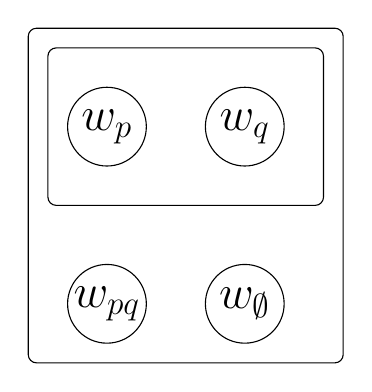
\begin{tikzpicture}[every node/.style={font=\LARGE}]
                \draw (2.5,13.75) circle (0.5cm) node {$w_p$};
                \draw (4.25,13.75) circle (0.5cm) node {$w_q$};
                \draw (2.5,11.5) circle (0.5cm) node {$w_{pq}$};
                \draw (4.25,11.5) circle (0.5cm) node {$w_{\emptyset}$};
                \draw [rounded corners=3.0] (1.75,14.75) rectangle (5.25,12.75);
                \draw [rounded corners=3.0] (1.5,15) rectangle (5.5,10.75);
            \end{tikzpicture}%
        }
        \caption{$\vDash(p\vee q)$,$\vDash$}
        \label{fig:3a}
    \end{subfigure}
    \hfill
    \begin{subfigure}[b]{0.23\textwidth}
        \centering
        \resizebox{\linewidth}{!}{%
            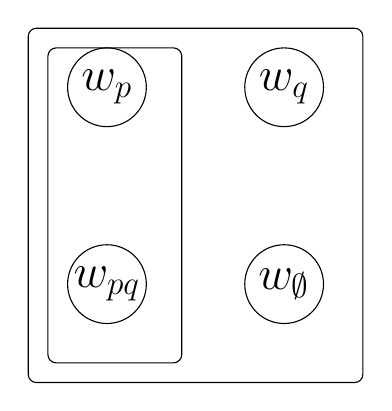
\begin{tikzpicture}[every node/.style={font=\LARGE}]
                \draw (0.75,14.25) circle (0.5cm) node {$w_p$};
                \draw (3,14.25) circle (0.5cm) node {$w_q$};
                \draw (0.75,11.75) circle (0.5cm) node {$w_{pq}$};
                \draw (3,11.75) circle (0.5cm) node {$w_{\emptyset}$};
                \draw [rounded corners=3.0] (0,14.75) rectangle (1.7,10.75);
                \draw [rounded corners=3.0] (-0.25,15) rectangle (4,10.5);
            \end{tikzpicture}%
        }
        \caption{Example 3b}
        \label{fig:3b}
    \end{subfigure}
    \hfill
    \begin{subfigure}[b]{0.23\textwidth}
        \centering
        \resizebox{\linewidth}{!}{%
            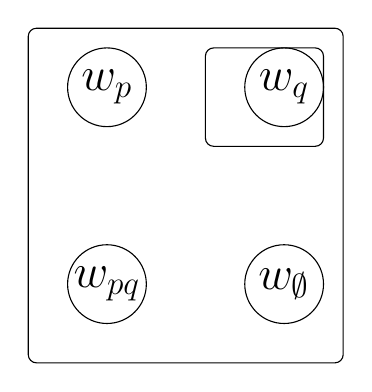
\begin{tikzpicture}[every node/.style={font=\LARGE}]
                \draw (0.75,14.25) circle (0.5cm) node {$w_p$};
                \draw (3,14.25) circle (0.5cm) node {$w_q$};
                \draw (0.75,11.75) circle (0.5cm) node {$w_{pq}$};
                \draw (3,11.75) circle (0.5cm) node {$w_{\emptyset}$};
                \draw [rounded corners=3.0] (2,14.75) rectangle (3.5,13.5);
                \draw [rounded corners=3.0] (-0.25,15) rectangle (3.75,10.75);
            \end{tikzpicture}%
        }
        \caption{Example 3c}
        \label{fig:3c}
    \end{subfigure}
    \hfill
    \begin{subfigure}[b]{0.23\textwidth}
        \centering
        \resizebox{\linewidth}{!}{%
            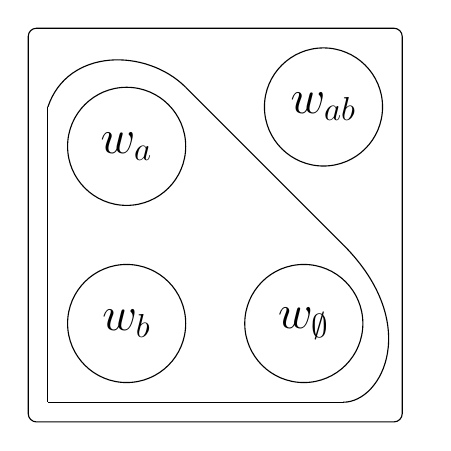
\begin{tikzpicture}[every node/.style={font=\LARGE}]
                \draw  (-8.75,5) circle (0.75cm) node {\LARGE $w_a$} ;
                \draw  (-8.75,2.75) circle (0.75cm) node {\LARGE $w_b$} ;
                \draw  (-6.25,5.5) circle (0.75cm) node {\LARGE $w_{ab}$} ;
                \draw  (-6.5,2.75) circle (0.75cm) node {\LARGE $w_{\emptyset}$} ;
                \draw [short] (-9.75,5.5) -- (-9.75,1.75);
                \draw [short] (-9.75,1.75) -- (-6,1.75);
                \draw [short] (-6,1.75) .. controls (-5.5,1.75) and (-5,2.75) .. (-6,3.75);
                \draw [short] (-6,3.75) -- (-8,5.75);
                \draw [short] (-9.75,5.5) .. controls (-9.5,6.25) and (-8.5,6.25) .. (-8,5.75);
                \draw [rounded corners = 3] (-10,6.5) rectangle (-5.25,1.5);
            \end{tikzpicture}%
        }
        \caption{Example 3d}
        \label{fig:3d}
    \end{subfigure}
    \caption{}
    \label{fig:all}
\end{figure}
\subsection{Free-Choice inference}
The way FC-inference is now modelled, is that given a formula/statement like $\lozenge (\alpha \lor \beta)$ in $\mathrm{ML}$, we enrich it to obtain a formula $\mathrm{BSML}$:
\[
    [\lozenge (\alpha \lor \beta)]^+ = \lozenge ((\alpha \land \texttt{NE}) \lor (\beta \land \texttt{NE})) \land \texttt{NE}
\]
This formula more accurately represents the meaning of a sentence in linguistics, given speakers' distaste for null verification.
To accurately model FC, we should then be able to infer $\lozenge \alpha \land \lozenge \beta$ from $[\lozenge (\alpha \lor \beta)]^+$.

-- Insert QuickCheck test to show this holds

\input{lib/lexer.lhs}


\input{lib/Parser.ly}

\input{exec/Main.lhs}

\section{Natural Deduction}

\section{Future work}
-- Efficiency\\
-- Proof search

\addcontentsline{toc}{section}{Bibliography}
\bibliographystyle{alpha}
\bibliography{references.bib}

\end{document}
